\hypertarget{Helpers_8c}{
\section{Helpers.c File Reference}
\label{Helpers_8c}\index{Helpers.c@{Helpers.c}}
}
{\tt \#include \char`\"{}coin\_\-common.h\char`\"{}}\par


Include dependency graph for Helpers.c:\nopagebreak
\begin{figure}[H]
\begin{center}
\leavevmode
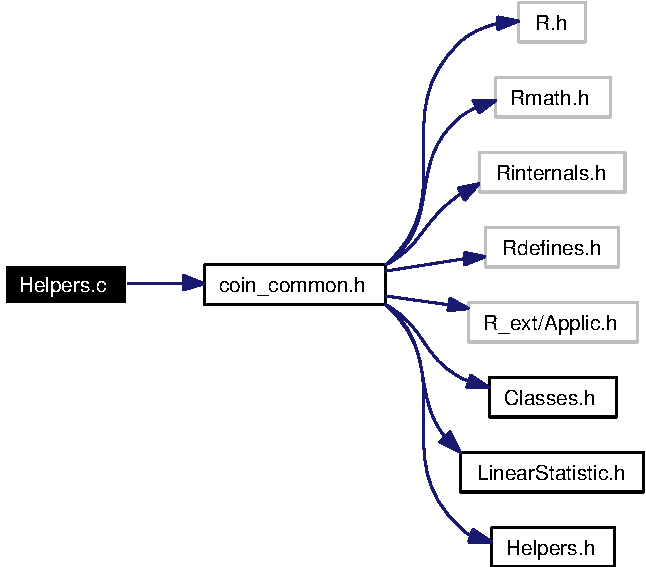
\includegraphics[width=350pt]{Helpers_8c__incl}
\end{center}
\end{figure}
\subsection*{Functions}
\begin{CompactItemize}
\item 
int \hyperlink{Helpers_8c_eeb672a71c45ead28b7b354414f2427a}{nrow} (SEXP x)
\item 
int \hyperlink{Helpers_8c_f1f46cc3e98630497a1ccb21d943fe65}{ncol} (SEXP x)
\item 
void \hyperlink{Helpers_8c_f7c710920d1496d23fdabad9b1d0e18c}{C\_\-SampleNoReplace} (int $\ast$x, int m, int k, int $\ast$ans)
\item 
SEXP \hyperlink{Helpers_8c_877d7b2378274b833a8c14b27d7a16a1}{R\_\-blocksetup} (SEXP block)
\item 
void \hyperlink{Helpers_8c_7c6b9e02fb5bcf919c7823d497cab062}{C\_\-blockperm} (SEXP blocksetup, int $\ast$ans)
\item 
SEXP \hyperlink{Helpers_8c_c97588ec77f215433b2933e5632f810d}{R\_\-blockperm} (SEXP block)
\item 
SEXP \hyperlink{Helpers_8c_140f9859faf864060c8a8ae129bc0190}{R\_\-MonteCarloIndependenceTest} (SEXP x, SEXP y, SEXP block, SEXP B)
\item 
SEXP \hyperlink{Helpers_8c_712dc63828d311dc3be30182fccf6f0f}{R\_\-maxstattrafo} (SEXP x, SEXP cutpoints)
\end{CompactItemize}


\subsection{Detailed Description}
Some additional functionality for package `coin'

\begin{Desc}
\item[Author:]\begin{Desc}
\item[Author]\end{Desc}
\end{Desc}
\begin{Desc}
\item[Date:]\begin{Desc}
\item[Date]\end{Desc}
\end{Desc}


Definition in file \hyperlink{Helpers_8c-source}{Helpers.c}.

\subsection{Function Documentation}
\hypertarget{Helpers_8c_7c6b9e02fb5bcf919c7823d497cab062}{
\index{Helpers.c@{Helpers.c}!C_blockperm@{C\_\-blockperm}}
\index{C_blockperm@{C\_\-blockperm}!Helpers.c@{Helpers.c}}
\subsubsection{\setlength{\rightskip}{0pt plus 5cm}void C\_\-blockperm (SEXP {\em blocksetup}, int $\ast$ {\em ans})}}
\label{Helpers_8c_7c6b9e02fb5bcf919c7823d497cab062}


Block permutation \begin{Desc}
\item[Parameters:]
\begin{description}
\item[{\em blocksetup}]as computed by `R\_\-blocksetup' \item[{\em ans}]integer vector \end{description}
\end{Desc}


Definition at line 110 of file Helpers.c.

References C\_\-SampleNoReplace().

Referenced by R\_\-blockperm(), and R\_\-MonteCarloIndependenceTest().

Here is the call graph for this function:\nopagebreak
\begin{figure}[H]
\begin{center}
\leavevmode
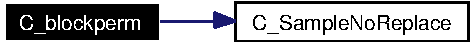
\includegraphics[width=139pt]{Helpers_8c_7c6b9e02fb5bcf919c7823d497cab062_cgraph}
\end{center}
\end{figure}
\hypertarget{Helpers_8c_f7c710920d1496d23fdabad9b1d0e18c}{
\index{Helpers.c@{Helpers.c}!C_SampleNoReplace@{C\_\-SampleNoReplace}}
\index{C_SampleNoReplace@{C\_\-SampleNoReplace}!Helpers.c@{Helpers.c}}
\subsubsection{\setlength{\rightskip}{0pt plus 5cm}void C\_\-SampleNoReplace (int $\ast$ {\em x}, int {\em m}, int {\em k}, int $\ast$ {\em ans})}}
\label{Helpers_8c_f7c710920d1496d23fdabad9b1d0e18c}


compute a permutation of a (random subset of) 0:(m-1) \begin{Desc}
\item[Parameters:]
\begin{description}
\item[{\em x}]an integer vector of length m \item[{\em m}]integer \item[{\em k}]integer \item[{\em ans}]an integer vector of length k \end{description}
\end{Desc}


Definition at line 42 of file Helpers.c.

Referenced by C\_\-blockperm().\hypertarget{Helpers_8c_f1f46cc3e98630497a1ccb21d943fe65}{
\index{Helpers.c@{Helpers.c}!ncol@{ncol}}
\index{ncol@{ncol}!Helpers.c@{Helpers.c}}
\subsubsection{\setlength{\rightskip}{0pt plus 5cm}int ncol (SEXP {\em x})}}
\label{Helpers_8c_f1f46cc3e98630497a1ccb21d943fe65}




Definition at line 22 of file Helpers.c.

Referenced by R\_\-ExpectCovarInfluence(), R\_\-ExpectCovarLinearStatistic(), R\_\-kronecker(), R\_\-LinearStatistic(), R\_\-MonteCarloIndependenceTest(), and R\_\-PermutedLinearStatistic().\hypertarget{Helpers_8c_eeb672a71c45ead28b7b354414f2427a}{
\index{Helpers.c@{Helpers.c}!nrow@{nrow}}
\index{nrow@{nrow}!Helpers.c@{Helpers.c}}
\subsubsection{\setlength{\rightskip}{0pt plus 5cm}int nrow (SEXP {\em x})}}
\label{Helpers_8c_eeb672a71c45ead28b7b354414f2427a}




Definition at line 11 of file Helpers.c.

Referenced by R\_\-ExpectCovarInfluence(), R\_\-ExpectCovarLinearStatistic(), R\_\-kronecker(), R\_\-LinearStatistic(), R\_\-MonteCarloIndependenceTest(), and R\_\-PermutedLinearStatistic().\hypertarget{Helpers_8c_c97588ec77f215433b2933e5632f810d}{
\index{Helpers.c@{Helpers.c}!R_blockperm@{R\_\-blockperm}}
\index{R_blockperm@{R\_\-blockperm}!Helpers.c@{Helpers.c}}
\subsubsection{\setlength{\rightskip}{0pt plus 5cm}SEXP R\_\-blockperm (SEXP {\em block})}}
\label{Helpers_8c_c97588ec77f215433b2933e5632f810d}




Definition at line 139 of file Helpers.c.

References C\_\-blockperm(), and R\_\-blocksetup().

Here is the call graph for this function:\nopagebreak
\begin{figure}[H]
\begin{center}
\leavevmode
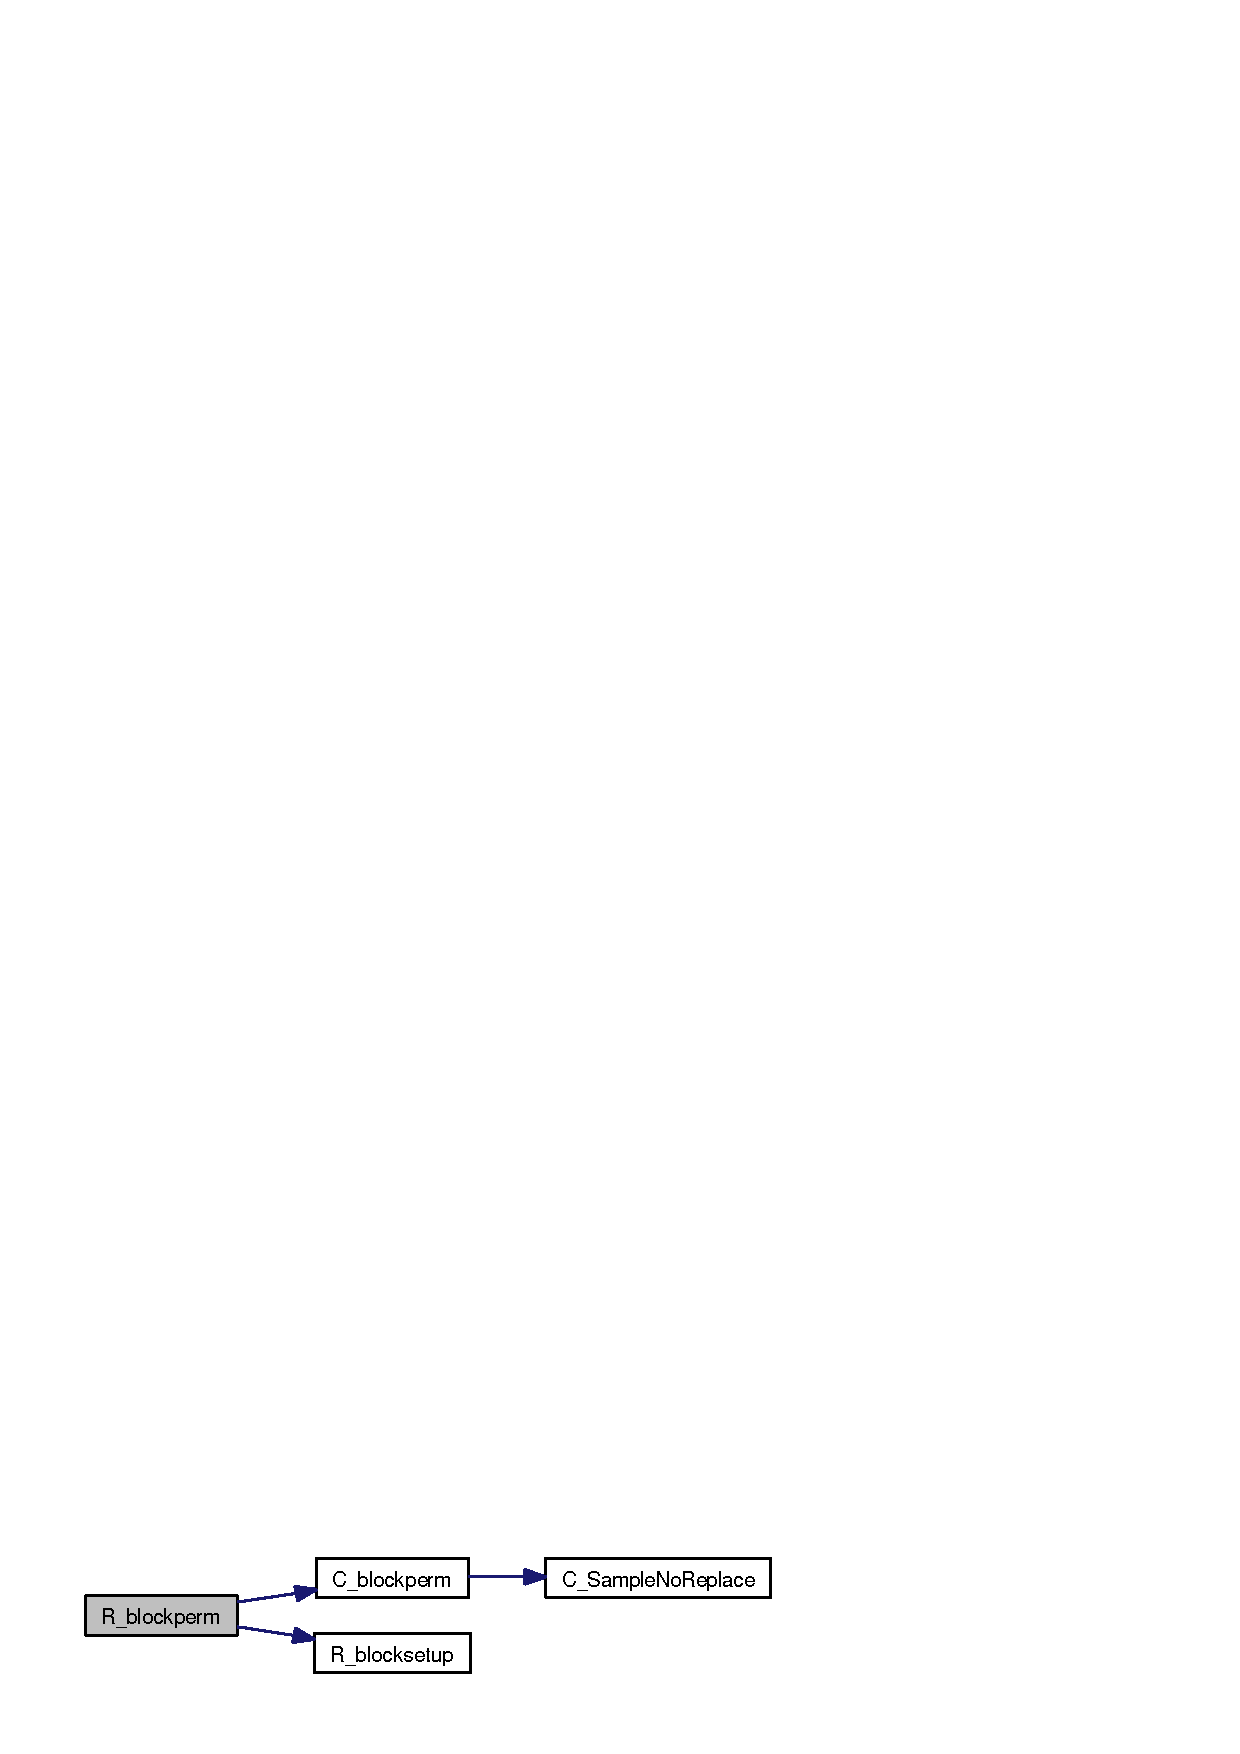
\includegraphics[width=196pt]{Helpers_8c_c97588ec77f215433b2933e5632f810d_cgraph}
\end{center}
\end{figure}
\hypertarget{Helpers_8c_877d7b2378274b833a8c14b27d7a16a1}{
\index{Helpers.c@{Helpers.c}!R_blocksetup@{R\_\-blocksetup}}
\index{R_blocksetup@{R\_\-blocksetup}!Helpers.c@{Helpers.c}}
\subsubsection{\setlength{\rightskip}{0pt plus 5cm}SEXP R\_\-blocksetup (SEXP {\em block})}}
\label{Helpers_8c_877d7b2378274b833a8c14b27d7a16a1}




Definition at line 56 of file Helpers.c.

Referenced by R\_\-blockperm(), and R\_\-MonteCarloIndependenceTest().\hypertarget{Helpers_8c_712dc63828d311dc3be30182fccf6f0f}{
\index{Helpers.c@{Helpers.c}!R_maxstattrafo@{R\_\-maxstattrafo}}
\index{R_maxstattrafo@{R\_\-maxstattrafo}!Helpers.c@{Helpers.c}}
\subsubsection{\setlength{\rightskip}{0pt plus 5cm}SEXP R\_\-maxstattrafo (SEXP {\em x}, SEXP {\em cutpoints})}}
\label{Helpers_8c_712dc63828d311dc3be30182fccf6f0f}




Definition at line 204 of file Helpers.c.\hypertarget{Helpers_8c_140f9859faf864060c8a8ae129bc0190}{
\index{Helpers.c@{Helpers.c}!R_MonteCarloIndependenceTest@{R\_\-MonteCarloIndependenceTest}}
\index{R_MonteCarloIndependenceTest@{R\_\-MonteCarloIndependenceTest}!Helpers.c@{Helpers.c}}
\subsubsection{\setlength{\rightskip}{0pt plus 5cm}SEXP R\_\-MonteCarloIndependenceTest (SEXP {\em x}, SEXP {\em y}, SEXP {\em block}, SEXP {\em B})}}
\label{Helpers_8c_140f9859faf864060c8a8ae129bc0190}




Definition at line 152 of file Helpers.c.

References C\_\-blockperm(), C\_\-PermutedLinearStatistic(), ncol(), nrow(), and R\_\-blocksetup().

Here is the call graph for this function:\nopagebreak
\begin{figure}[H]
\begin{center}
\leavevmode
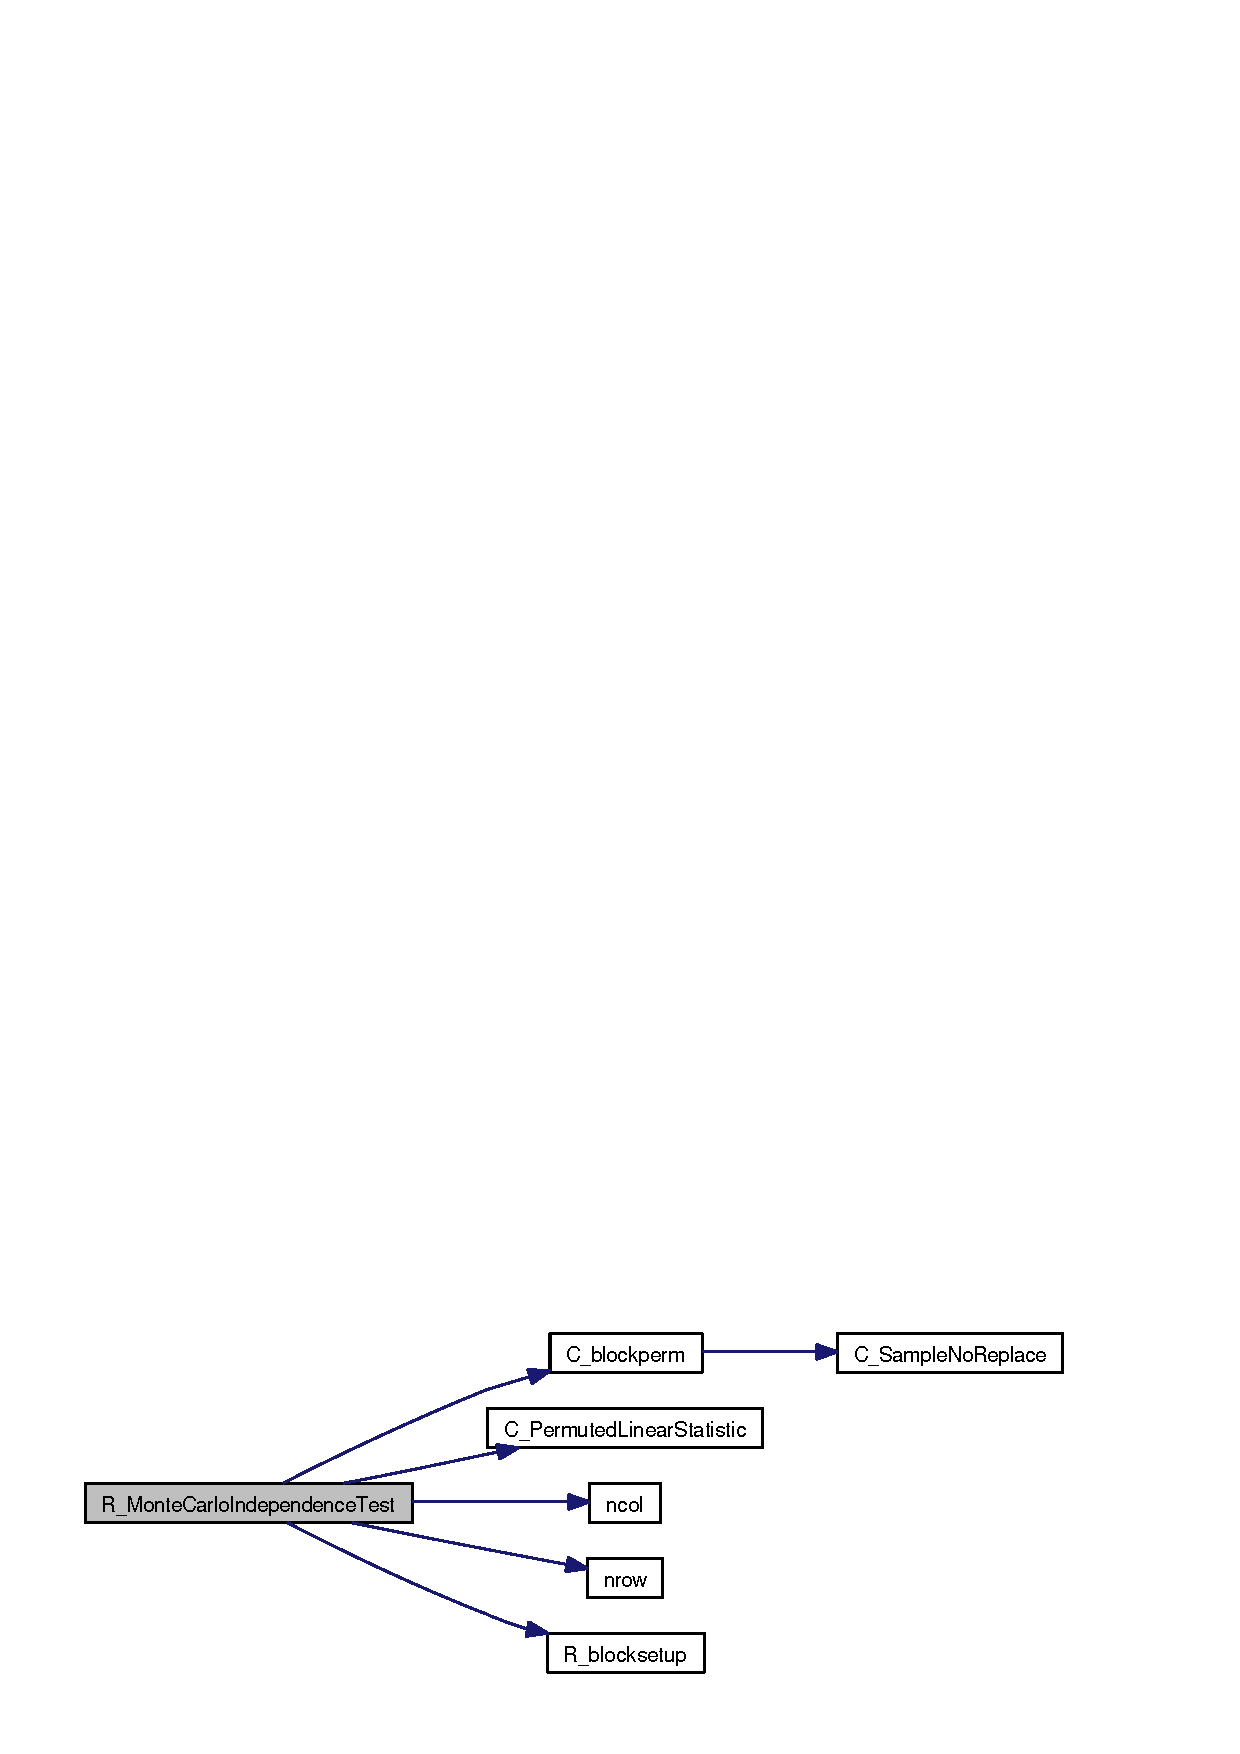
\includegraphics[width=277pt]{Helpers_8c_140f9859faf864060c8a8ae129bc0190_cgraph}
\end{center}
\end{figure}
